%\setmainfont{Noteworthy}
%TODO: provide your details here.
\begin{frame}
    \frametitle{About Your Fellows}
    \begin{itemize}
        \item Hi there! We are \textcolor{blue}{\textbf{ Mohid Faisal}  \textcolor{black}{and}\textbf{ Muhammad Wasif}}.
        \item We are Associate Students at ITU.
    \end{itemize}
\end{frame}




\begin{frame}
    \frametitle{Recap: High School Multiplication Algorithm}
    \centering
    \textbf{Time Complexity Analysis:}
    \begin{itemize}
        \item Let \( n \) be the number of digits.
        \item There are \( n^2 \) digit multiplications.
        \item Addition and carry operations take at most \( O(n) \).
        \item Overall, the time complexity is \( O(n^2) \).
    \end{itemize}
    
    \vspace{0.5cm}
    \centering\textbf{\textcolor{red}{Can we do better?}}
\end{frame}

\begin{frame}
    \frametitle{Karatsuba Multiplication Algorithm}
    \vspace{0.3cm} 
    \textbf{Karatsuba Algorithm} $\rightarrow$ the divide and conquer algorithm for Integer Multiplication
    
    \vspace{0.3cm}
    \textbf{Approach:}
    \begin{itemize}
        \item Given two binary numbers: \( X = 0011101010 \), \( Y = 1010000101 \).
        \item Split them into two halves:
        \begin{itemize}
            \item $X_h = \underline{00111}$, $X_l = \underline{01010}$
            \item $Y_h = \underline{10100}$, $Y_l = \underline{00101}$
        \end{itemize}
        \item Reconstruct:
        \begin{itemize}
            \item $X = 2^{n/2} \times \underline{X_h} + \underline{X_l}$
            \item $Y = 2^{n/2} \times \underline{Y_h} + \underline{Y_l}$
        \end{itemize}
        \item Multiply using:
        \begin{equation*}
            X \cdot Y = ( 2^{n/2} \underline{X_h} + \underline{X_l} ) \cdot ( 2^{n/2} \underline{Y_h} + \underline{Y_l} )
        \end{equation*}
        \begin{equation*}
            = 2^n \underline{X_h Y_h} + 2^{n/2} \underline{X_h Y_l} + 2^{n/2} \underline{Y_h X_l} + \underline{X_l Y_l}
        \end{equation*}
        \item Next, we compute the smaller multiplications recursively and then add up the results along with bit shifts to get the final product.
    \end{itemize}
\end{frame}

\begin{frame}
    \frametitle{Karatsuba Multiplication Algorithm - Explanation}

    \textbf{Algorithm Overview}  

    Given two numbers \( X \) and \( Y \), the algorithm follows these steps:

    1. If the number of bits is small (base case), multiply directly.
    
    2. Split \( X \) into two halves: higher bits \( X_h \) and lower bits \( X_l \).
    
    3. Split \( Y \) into two halves: higher bits \( Y_h \) and lower bits \( Y_l \).
    
    4. Recursively compute:
       \[
       hh = X_h \times Y_h
       \]
       \[
       hl = X_h \times Y_l
       \]
       \[
       lh = X_l \times Y_h
       \]
       \[
       ll = X_l \times Y_l
       \]

    5. Combine the results using bit shifts:
       \[
       X \times Y = (2^n \times hh) + (2^{n/2} \times (hl + lh)) + ll
       \]

    \textbf{Recurrence Relation:}
    \begin{equation*}
        T(n) = 4T(n/2) + O(n)
    \end{equation*}

    \textbf{By Master Theorem:}
    \begin{equation*}
        T(n) = \Theta(n^2)
    \end{equation*}

\end{frame}



\begin{frame}
    \frametitle{Gauss's Insight}

    Gauss observed that the product of two complex numbers \( (a + bi) \cdot (c + di) \) can be computed using only three multiplications instead of the naive four. Specifically:

    \[
    (a + bi) \cdot (c + di) = (ac - bd) + (ad + bc)i
    \]

    \vspace{0.5cm}

    This can be rewritten using three multiplications:

    \begin{itemize}
        \item Compute \( ac \).
        \item Compute \( bd \).
        \item Compute \( (a + b)(c + d) \).
    \end{itemize}

    \vspace{0.5cm}

    Then, the term \( ad + bc \) can be derived as:

    \[
    ad + bc = (a + b)(c + d) - ac - bd
    \]

    \vspace{0.5cm}

    This reduces the number of multiplications from 4 to 3.
\end{frame}







\begin{frame}
    \frametitle{Optimization of Algorithm}

    \textbf{We can do some algebra to express the multiplication that will require fewer recursive calls and give us a better big-O bound.}

    \vspace{0.5cm}

    \[
    \underline{X} \cdot \underline{Y} = ( 2^{n/2} \underline{X_h} + \underline{X_l} ) \cdot ( 2^{n/2} \underline{Y_h} + \underline{Y_l} )
    \]

    \[
    = 2^n \underline{X_h Y_h} + 2^{n/2} \underline{X_h Y_l} + 2^{n/2} \underline{Y_h X_l} + \underline{X_l Y_l}
    \]

    \vspace{0.5cm}

    \textbf{Note that:}

    \[
    ( \underline{X_h} + \underline{X_l} ) \cdot ( \underline{Y_h} + \underline{Y_l} ) = \underline{X_h Y_h} + ( \underline{X_h Y_l} + \underline{X_l Y_h} ) + \underline{X_l Y_l}
    \]

    \vspace{0.3cm}

    \textbf{Thus:}

    \[
    \underline{X_h Y_l} + \underline{X_l Y_h} = ( \underline{X_h} + \underline{X_l} ) \cdot ( \underline{Y_h} + \underline{Y_l} ) - \underline{X_h Y_h} - \underline{X_l Y_l}
    \]

    \vspace{0.5cm}

    \textbf{Now, instead of four recursive calls, we will make three recursive calls.}

\end{frame}

\begin{frame}
    \frametitle{Optimized Karatsuba Algorithm}

    The optimization reduces the number of recursive calls from 4 to 3 by computing:

    \[
    X \cdot Y = (2^{n/2} X_h + X_l) \cdot (2^{n/2} Y_h + Y_l)
    \]

    Expanding and rearranging using Gauss's trick:

    \[
    X \cdot Y = 2^n X_h Y_h + 2^{n/2} (X_h Y_l + X_l Y_h) + X_l Y_l
    \]

    Instead of computing \( X_h Y_l \) and \( X_l Y_h \) separately, we compute:

    \[
    P = (X_h + X_l) \cdot (Y_h + Y_l)
    \]

    Then, we derive:

    \[
    X_h Y_l + X_l Y_h = P - X_h Y_h - X_l Y_l
    \]

    \vspace{0.1cm}
    \textbf{Optimized Recurrence Relation:}
    \[
        T(n) = 3T(n/2) + O(n)
    \]

    \textbf{By Master Theorem:}
    \[
        T(n) = \Theta(n^{\log_2 3})
    \]

\end{frame}


\begin{frame}
    \frametitle{Karatsuba Multiplication - Visual Representation}
    \centering
    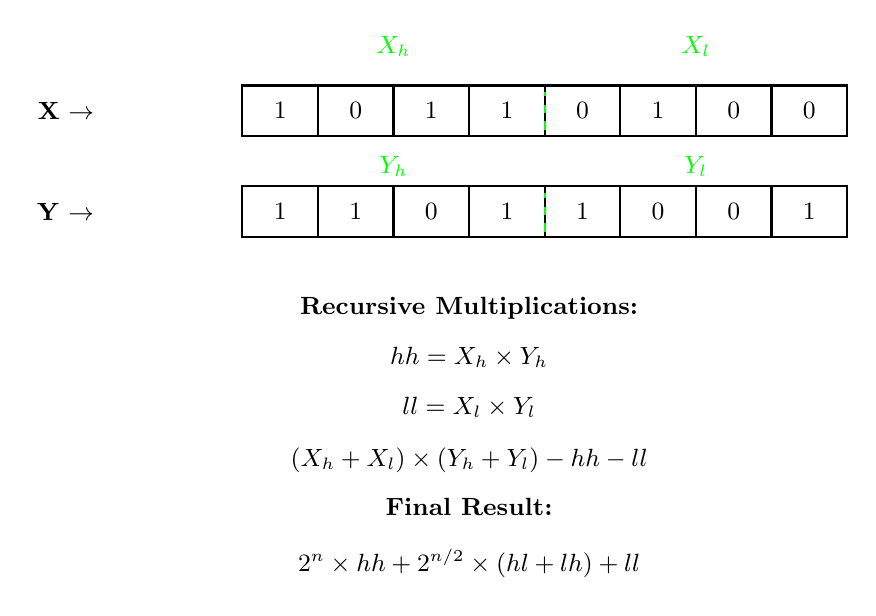
\begin{tikzpicture}[scale=0.8, every node/.style={font=\small}]
        % Define positions
        \def\xstart{2}
        \def\ystart{0}
        \def\width{1.2}  % Box width
        \def\height{0.8} % Box height
        \def\gap{0.2}    % Gap between splits

        % Binary numbers
        \node[left] at (\xstart-1, \ystart+0.5*\height) {\textbf{X} $\rightarrow$};
        \node[left] at (\xstart-1, \ystart-1.5*\height) {\textbf{Y} $\rightarrow$};

        % X number
        \foreach \i [count=\j] in {1,0,1,1,0,1,0,0} {
            \draw[thick] (\xstart+\j*\width, \ystart) rectangle ++(\width, \height);
            \node at (\xstart+\j*\width+0.5*\width, \ystart+0.5*\height) {\i};
        }

        % Y number (below X)
        \foreach \i [count=\j] in {1,1,0,1,1,0,0,1} {
            \draw[thick] (\xstart+\j*\width, \ystart-2*\height) rectangle ++(\width, \height);
            \node at (\xstart+\j*\width+0.5*\width, \ystart-2*\height+0.5*\height) {\i};
        }

        % Adjusted partitioning exactly at the 4th block boundary
        \draw[dashed, green, thick] (\xstart+5*\width, \ystart+0.1) -- (\xstart+5*\width, \ystart+\height-0.1);
        \draw[dashed, green, thick] (\xstart+5*\width, \ystart-1.9*\height) -- (\xstart+5*\width, \ystart-2*\height+\height-0.1);

        % Labels for high and low parts
        \node[green, above] at (\xstart+3*\width, \ystart+\height+0.3) {$X_h$};
        \node[green, above] at (\xstart+7*\width, \ystart+\height+0.3) {$X_l$};

        \node[green, above] at (\xstart+3*\width, \ystart-1*\height) {$Y_h$};
        \node[green, above] at (\xstart+7*\width, \ystart-1*\height) {$Y_l$};

        % Recursive Calls
        \node[below] at (\xstart+4*\width, \ystart-3*\height) {\textbf{Recursive Multiplications:}};
        \node[below] at (\xstart+4*\width, \ystart-4*\height) {$hh = X_h \times Y_h$};
        \node[below] at (\xstart+4*\width, \ystart-5*\height) {$ll = X_l \times Y_l$};
        \node[below] at (\xstart+4*\width, \ystart-6*\height) {$(X_h+X_l) \times (Y_h+Y_l) - hh - ll$};

        % Final result combination
        \node[below] at (\xstart+4*\width, \ystart-7*\height) {\textbf{Final Result:}};
        \node[below] at (\xstart+4*\width, \ystart-8*\height) {$2^n \times hh + 2^{n/2} \times (hl+lh) + ll$};
    \end{tikzpicture}
\end{frame}

\begin{frame}{Time Complexity Comparison}

  \begin{columns}
      % Left column for legend (key)
      \column{0.3\textwidth}
      \textbf{Multiplication Algorithms:}
      \begin{itemize}
          \item \textcolor{red}{$O(n^2)$} - High School Method
          \item \textcolor{green}{$O(n^{1.585})$} - Karatsuba Algorithm
      \end{itemize}

      % Right column for graph
      \column{0.7\textwidth}
      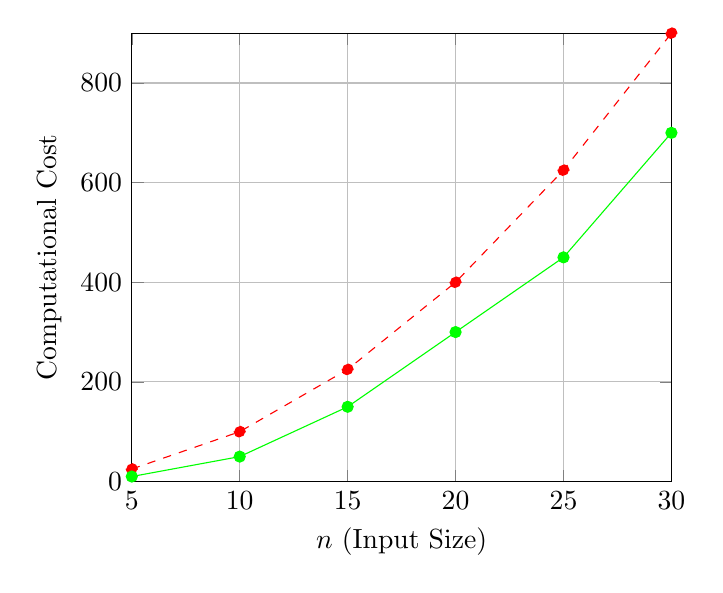
\begin{tikzpicture}
          \begin{axis}[
              xlabel={$n$ (Input Size)},
              ylabel={Computational Cost},
              xmin=5, xmax=30,
              ymin=0, ymax=900,
              grid=major
          ]
          
          % Red Curve (O(n^2)) - High School Algorithm
          \addplot[red, mark=*, dashed] coordinates {
              (5, 25) (10, 100) (15, 225) (20, 400) (25, 625) (30, 900)
          };
          
          % Purple Curve (O(n^1.585)) - Karatsuba Algorithm
          \addplot[green, mark=*, solid] coordinates {
              (5, 10) (10, 50) (15, 150) (20, 300) (25, 450) (30, 700)
          };

          \end{axis}
      \end{tikzpicture}
  \end{columns}
\end{frame}

\begin{frame}
    \frametitle{Strassen's Matrix Multiplication}

    \textbf
    Strassen’s algorithm is a \textbf{divide-and-conquer} approach for matrix multiplication that is asymptotically faster than the conventional method. It reduces the number of multiplications required, improving efficiency.

    \vspace{0.5cm}
    \textbf{Standard Matrix Multiplication:}  
    For two \( n \times n \) matrices \( A \) and \( B \), the traditional matrix multiplication requires:
    
    \begin{itemize}
        \item \( O(n^3) \) scalar multiplications.
        \item \( O(n^3) \) scalar additions.
    \end{itemize}

\end{frame}

\begin{frame}
    \frametitle{Strassen’s Approach}

    \textbf  
    Strassen’s algorithm breaks down the multiplication process using \textbf{divide and conquer} and reduces the number of scalar multiplications.

    \vspace{0.5cm}
    \textbf{Step 1: Divide the Matrices}  
    For two \( n \times n \) matrices \( A \) and \( B \), split each into four \( \frac{n}{2} \times \frac{n}{2} \) submatrices:

    \[
    A =
    \begin{bmatrix}
        \textcolor{red}{A_{11}} & \textcolor{red}{A_{12}} \\
        \textcolor{red}{A_{21}} & \textcolor{red}{A_{22}}
    \end{bmatrix}
    , \quad
    B =
    \begin{bmatrix}
        \textcolor{red}{B_{11}} & \textcolor{red}{B_{12}} \\
        \textcolor{red}{B_{21}} & \textcolor{red}{B_{22}}
    \end{bmatrix}
    \]

    where each \( \textcolor{red}{A_{ij}} \) and \( \textcolor{red}{B_{ij}} \) is of size \( \frac{n}{2} \times \frac{n}{2} \).

    
\end{frame}

\begin{frame}
    \frametitle{Strassen’s Algorithm: Recursive Multiplications}

    \textbf{Step 2: Compute 7 Recursive Multiplications}  
    Instead of directly computing the 8 matrix products, Strassen defined 7 intermediate matrix products:

   \[
    M_1 = (\textcolor{red}{A_{11}} + \textcolor{red}{A_{22}}) (\textcolor{red}{B_{11}} + \textcolor{red}{B_{22}})
\]
\[
    M_2 = (\textcolor{red}{A_{21}} + \textcolor{red}{A_{22}}) \textcolor{red}{B_{11}}
\]
\[
    M_3 = \textcolor{red}{A_{11}} (\textcolor{red}{B_{12}} - \textcolor{red}{B_{22}})
\]
\[
    M_4 = \textcolor{red}{A_{22}} (\textcolor{red}{B_{21}} - \textcolor{red}{B_{11}})
\]
\[
    M_5 = (\textcolor{red}{A_{11}} + \textcolor{red}{A_{12}}) \textcolor{red}{B_{22}}
\]
\[
    M_6 = (\textcolor{red}{A_{21}} - \textcolor{red}{A_{11}}) (\textcolor{red}{B_{11}} + \textcolor{red}{B_{12}})
\]
\[
    M_7 = (\textcolor{red}{A_{12}} - \textcolor{red}{A_{22}}) (\textcolor{red}{B_{21}} + \textcolor{red}{B_{22}})
\]


\end{frame}

\begin{frame}
    \frametitle{Strassen’s Algorithm: Compute Result Matrix}

    \textbf{Step 3: Compute the Result Matrix}  
    Using the intermediate results, we compute the submatrices of \( C \):

    \[
    \textcolor{red}{C_{11}} = M_1 + M_4 - M_5 + M_7
\]
\[
    \textcolor{red}{C_{12}} = M_3 + M_5
\]
\[
    \textcolor{red}{C_{21}} = M_2 + M_4
\]
\[
    \textcolor{red}{C_{22}} = M_1 - M_2 + M_3 + M_6
\]


\end{frame}

\begin{frame}
    \frametitle{Time Complexity Analysis}

    Strassen's method reduces the number of multiplications from 8 to 7, but it increases the number of additions and subtractions.

    \textbf{Recurrence Relation:}
    \[
    T(n) = 7T(n/2) + O(n^2)
    \]

    \textbf{Solving using the Master Theorem:}
    \[
    T(n) = O(n^{\log_2 7}) \approx O(n^{2.81})
    \]

    This is faster than the standard matrix multiplication complexity of \( O(n^3) \).
\end{frame}


\begin{frame}
  \frametitle{The Secretary Problem: Background and Rules}
  
  During WWII, new treatments were often tested on human subjects to determine their effectiveness. Researchers grappled with a critical question: when was the optimal point to stop testing and adopt a treatment? This dilemma inspired the Secretary Problem (or Optimal Stopping Problem) in computer science—deciding the best moment to stop searching among sequentially presented options to maximize the chance of selecting the best one.
  \begin{block}{Rules}
      \begin{itemize}
        \item Candidates are interviewed one at a time in a random order.
        \item You must decide immediately after each interview.
        \item Once a candidate is rejected, you cannot go back and hire them.
        \item Only one candidate can be selected.
        \item The objective is to choose the best candidate overall.
      \end{itemize}
    \end{block}  
\end{frame}



  \begin{frame}
      \frametitle{The Secretary Problem: Algorithm}
      \begin{columns}[t]
        \column{0.5\textwidth}
          \begin{block}{Algorithm}
            \begin{enumerate}
              \item Determine the total number of candidates (n).
              \item Interview the first $k$ candidates and record the best candidate seen ($x$).
              \item For each candidate from $k+1$ to $n$, if a candidate is better than $x$, hire them immediately and stop.
              \item If no candidate after the observation phase is better, select the last candidate.
            \end{enumerate}
          \end{block}
        \column{0.5\textwidth}
          \centering
          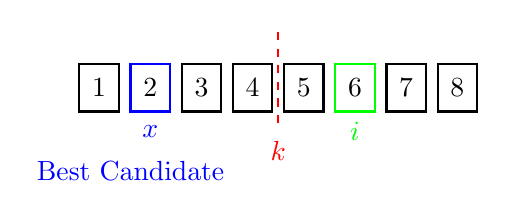
\begin{tikzpicture}[scale=0.5]
            % Parameters for visualization
            \def\n{8}         % Total number of candidates (example: 8)
            \def\width{1}     % Width of each rectangle
            \def\height{1.2}  % Height of each rectangle
            \def\gap{0.3}     % Gap between rectangles
            
            % Draw the array of candidate rectangles
            \foreach \i in {1,...,\n} {
              \draw[thick] ({(\i-1)*(\width+\gap)},0) rectangle ++(\width, \height);
              \node at ({(\i-1)*(\width+\gap)+0.5*\width}, {0.5*\height}) {\i};
            }
            
            % Mark the observation phase boundary at candidate k (assume k=3)
            \def\k{4}
            \draw[red, dashed, thick] ({\k*(\width+\gap)-\gap/2}, -0.3) -- ({\k*(\width+\gap)-\gap/2}, \height+0.9);
            \node[red] at ({\k*(\width+\gap)-\gap/2}, -1) {$k$};
    
            % Highlight the best candidate (x) among the first k (assume candidate 2 is best)
            \def\x{2}
            \draw[blue, thick] ({(\x-1)*(\width+\gap)}, 0) rectangle ++(\width, \height);
            \node[blue] at ({(\x-1)*(\width+\gap)+0.5*\width}, -0.5) {$x$};
            \node[blue] at ({(\x-1)*(\width*0.5+\gap)+0.5*\width}, -1.5) {Best Candidate};

            \def\x{6}
            \draw[green, thick] ({(\x-1)*(\width+\gap)}, 0) rectangle ++(\width, \height);
            \node[green] at ({(\x-1)*(\width+\gap)+0.5*\width}, -0.5) {$i$};

          \end{tikzpicture}
          \vspace*{3cm} % Adjust the space as needed to push the text toward the bottom
          {\color{red}\textbf{}}
          {\color{red}\textbf{}}
          {\color{red}\textbf{}}
          {\color{red}\textbf{Let's analyze! But before that…}}
          {\color{red}\textbf{Some Background of Probability.}}
      \end{columns}
    \end{frame}
    
    \begin{frame}
      \frametitle{Probability Background}
      \begin{columns}[T]
        \column{0.6\textwidth}
           \begin{block}{Uniform Probability: Definition}
    In a uniform probability model—where every outcome is equally likely—the probability of an event \(E\) is given by:
    \[
      P(E) = \frac{|E|}{|S|},
    \]
    where:
    \begin{itemize}
      \item \(|S|\) is the total number of outcomes (sample space).
      \item \(|E|\) is the number of favorable outcomes.
    \end{itemize}
    Consequently, for any outcome \(x\) in \(S\),
    \[
      P(x) = \frac{1}{|S|}.
    \]
  \end{block}
          
        \column{0.4\textwidth}
          \centering
          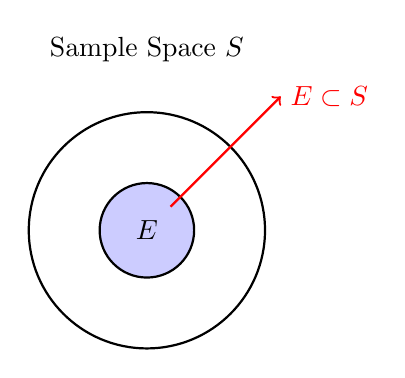
\begin{tikzpicture}[scale=1]
            % Draw the sample space as a circle
            \draw[thick] (0,0) circle (1.5cm);
            \node at (0,2.3) {Sample Space \(S\)};
            % Draw event E as an inner circle
            \draw[fill=blue!20, thick] (0,0) circle (0.6cm);
            \node at (0,0) {\(E\)};
            % Add an annotation arrow with text indicating E ⊂ S
            \draw[->, red, thick] (0.3,0.3) -- (1.7,1.7);
            \node[red, right] at (1.7,1.7) {\(E \subset S\)};
          \end{tikzpicture}
      \end{columns}
    \end{frame}
    
      \begin{frame}
          \frametitle{Probability Background}
        
      \begin{block}{Conditional Probability}
        The probability of an event \(E\) given that event \(F\) occurs [P(F)=1] is
        \[
          P(E \mid F) = \frac{P(E \cap F)}{P(F)}, \quad P(F) > 0.
        \] 
        \end{block}            
        \begin{block}{Independent Events} 
        Events \(E\) and \(F\) are independent if the occurrence of one does not depend on the other.
        \[
          \text{Since E and F are independent: }
          P(E) = P(E \mid F)
        \]
        and similarly
        \[
          P(F) = P(F \mid E)
        \]
      \end{block}
    
    \end{frame}

    \begin{frame}
      \frametitle{Probability of Optimal Hire}
      \centering
      \[
P(\text{OH}) = \text{we hire the best candidate}
\]
      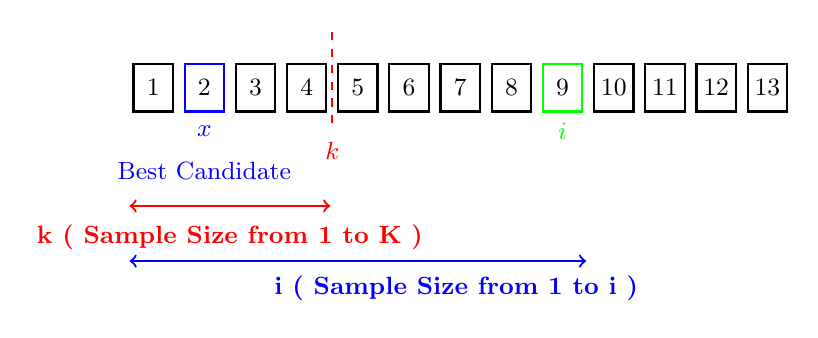
\begin{tikzpicture}[scale=0.5, every node/.style={font=\small}]
        % Parameters for visualization
        \def\n{13}         % Total number of candidates (example: 8)
        \def\width{1}     % Width of each rectangle
        \def\height{1.2}  % Height of each rectangle
        \def\gap{0.3}     % Gap between rectangles
        
        % Draw the array of candidate rectangles
        \foreach \i in {1,...,\n} {
          \draw[thick] ({(\i-1)*(\width+\gap)},0) rectangle ++(\width, \height);
          \node at ({(\i-1)*(\width+\gap)+0.5*\width}, {0.5*\height}) {\i};
        }
        
        % Mark the observation phase boundary at candidate k (assume k=4)
        \def\k{4}
        \draw[red, dashed, thick] ({\k*(\width+\gap)-\gap/2}, -0.3) -- ({\k*(\width+\gap)-\gap/2}, \height+0.9);
        \node[red] at ({\k*(\width+\gap)-\gap/2}, -1) {$k$};
        
        % Highlight the best candidate (x) among the first k (assume candidate 2 is best)
        \def\x{2}
        \draw[blue, thick] ({(\x-1)*(\width+\gap)}, 0) rectangle ++(\width, \height);
        \node[blue] at ({(\x-1)*(\width+\gap)+0.5*\width}, -0.5) {$x$};
        \node[blue] at ({(\x-1)*(\width+\gap)+0.5*\width}, -1.5) {Best Candidate};
        
        % Highlight candidate i in green (assume candidate 6)
        \def\iCandidate{9}
        \draw[green, thick] ({(\iCandidate-1)*(\width+\gap)}, 0) rectangle ++(\width, \height);
        \node[green] at ({(\iCandidate-1)*(\width+\gap)+0.5*\width}, -0.5) {$i$};
        
        % Draw region K as a double-headed arrow (red) below the array
\draw[<->, red, thick] (-0.1, -2.4) -- ({\k*(\width+\gap)-\gap+0.1}, -2.4);
\node[red] at ({(-0.1 + (\k*(\width+\gap)-\gap+0.1))/2}, -3.2) {\textbf{k ( Sample Size from 1 to K )}};

% Draw region I as a double-headed arrow (blue) below the array, shifted down to create space
\draw[<->, blue, thick] (-0.1, -3.8) -- ({\iCandidate*(\width+\gap)-\gap+0.1}, -3.8);
\node[blue] at ({((\k*(\width+\gap)-\gap) + (\iCandidate*(\width+\gap)-\gap+0.1))/2}, -4.5) {\textbf{i ( Sample Size from 1 to i )}};

      \end{tikzpicture}
      \[
        P(OH) = \sum_{i=k+1}^{n} \left( P(i\ \text{is best and we hire }i)   \right)
      \]

     \begin{itemize}
      \item Why use k+1 instead of 1?
     \end{itemize} 
     \[
P(\text{OH}) = 0, \text{Since we never hire the first k candidates}
\]


    \end{frame}

    \begin{frame}
      \frametitle{Probability of Optimal Hire}
      \centering
      \[
        P(OH_i) = i\ \text{is best and we hire }i
        \]
        \begin{itemize}
          \item \(B_i\): \(i\)-th candidate is the best
          \item \(O_i\): none of the applicants in \(\{k+1 \ldots i-1\}\) are picked
        \end{itemize}
      
        \[
          OH_i = B_i \;\land\; O_i
        \]
\[
P(\text{OH}_i)
= P\bigl(B_i \wedge O_i\bigr)
\]
\[
P(\text{OH}_i)
= P\bigl(B_i\bigr) \times \Pr\bigl(O_i \mid B_i\bigr)
\]
\begin{itemize}
\item Since \(B_i\) and \(O_i\) are independent:
\end{itemize}

\[
P(\text{OH}_i)
= P\bigl(B_i\bigr) \times P\bigl(O_i\bigr)
\]
    \end{frame}
\begin{frame}
\frametitle{Probability of Optimal Hire}
\centering
\[
P(B_i)= \frac{1}{n},      \text{     [Uniform Probability]}
\]
\[
  P(O_i)= \frac{k-1}{i-1}
  \]
  \[
P(\text{OH}_i)
= P\bigl(B_i\bigr) \times P\bigl(O_i\bigr)
\]
\[
P(\text{OH}_i)
= \frac{1}{n} \times \frac{k-1}{i-1}
\]
\[
P(\text{OH}) = \sum_{i=k+1}^{n} \left( \frac{1}{n} \times \frac{k-1}{i-1}   \right)
\]


\end{frame}
    \begin{frame}
      \frametitle{Maximum Probability of Optimal Hire}
      \begin{block}{Class Discussion}
        \begin{itemize}
          \item \textbf{Professor:} What is the best value of \(k\) to maximize the Probability of Optimal Hire?
          \item \textbf{Sharib:} \(k = \frac{n}{3}\).
          \item \textbf{Other students:} (suggested different values)
          \item \textbf{Professor:} We will find that in the next class. Time's up!
        \end{itemize}
      \end{block}
    \end{frame}
    
    